%=======================================================================
% CSE465 Final Report - OWMTL  |  FULL DRAFT v1  |  generated 2026-08-21
%
% Format rules: see paper_requirement.md.  Blank format skeleton: template_blank.tex
%
% HOW TO READ THIS DRAFT
%   Every number in this file was read from a committed results JSON in the
%   repository, or computed from a committed raw confusion matrix using
%   Asif's/audit/icbhi_score_audit.py's official_icbhi().  Nothing is invented.
%   Work that does not exist yet is marked with \pending{...} and renders in red.
%   Search for "pending" to find every remaining hole.
%=======================================================================
\documentclass[journal,onecolumn]{IEEEtran}

\usepackage{cite}
\usepackage{amsmath,amssymb}
\usepackage{graphicx}
\usepackage{booktabs}
\usepackage{multirow}
\usepackage{array}
\usepackage{xcolor}
\usepackage{tikz}
\usetikzlibrary{shapes.geometric,arrows.meta,positioning}
\usepackage{url}
\usepackage[hidelinks]{hyperref}

\graphicspath{{figures/}}

% Draft-only marker for work that is not done yet. DELETE the macro and every
% call before submission -- if any survive, they are impossible to miss in red.
\newcommand{\pending}[1]{\textcolor{red}{\textbf{[PENDING: #1]}}}

\newcommand{\best}[1]{\textbf{#1}}

\begin{document}

%=======================================================================
\title{Corrected Evaluation Baselines for Respiratory Sound\\
Classification on ICBHI 2017: Metric Inflation, Split\\
Provenance, and a Label-Reliability Ceiling}

\author{Asif~\pending{full name},
        Barshon~Basak,
        Farhana~\pending{full name},
        and~Sami~\pending{full name}%
\thanks{Department of Electrical and Computer Engineering, North South
University, Dhaka, Bangladesh. Course: CSE465, Section \pending{section}.
Supervisor: \pending{supervisor name}. E-mail: \pending{contact e-mail}.}}

\maketitle

%=======================================================================
\begin{abstract}
Respiratory sound classification on the ICBHI 2017 database has become a saturated
benchmark, with well over a hundred published systems reporting a single headline
score. This paper asks a prior question: how much of that score is a property of the
model, and how much is a property of how it was measured. We audit our own
multi-model respiratory sound pipeline and report three measurement faults, each
recovered from committed confusion matrices rather than asserted. First, a
macro-averaged variant of the challenge score inflated our results by an average of
eleven points across fifteen committed runs, and by twenty-two points at worst.
Second, a silently substituted patient-identifier rule produced a test partition of
eleven patients and seven percent of the respiratory cycles while being recorded as
the official sixty-forty split; the two architectures we have since evaluated on the
true split score roughly twenty points lower. Third, the published split assigns
recordings rather than patients, so two patients appear on both sides of it and it is
not patient independent as it is routinely described. We then report a pre-registered
validity gate for physics-derived acoustic concepts, run twice and failed twice, and
read that failure against published human performance on the same labels, where seven
senior physicians reach a score below fifty percent and twelve physicians agree on
detailed adventitious sound descriptions only poorly. We release the corrected split
loader, a canonical score format with paired significance tests, and the audit tool
that detects all three faults. The contribution is a measurement rather than a
mechanism: concept-level validation against these labels is bounded by the
reliability of the labels themselves.
\end{abstract}

\begin{IEEEkeywords}
Ablation study, deep learning, evaluation protocol, explainable artificial
intelligence, ICBHI 2017, label reliability, reproducibility, respiratory sound
classification, transfer learning, vision transformers.
\end{IEEEkeywords}

%=======================================================================
\section{Introduction}
\label{sec:intro}

Auscultation remains the first-line examination for respiratory disease, and it is
also one of the least reproducible. The acoustic events that clinicians listen
for---crackles and wheezes---are short, low-energy, and easily masked by heart
sounds, ambient noise, and stethoscope handling. Automating their detection is
therefore an attractive target, and the ICBHI 2017 Respiratory Sound Database has
become the field's default proving ground for it. We chose this problem because the
benchmark is mature enough that a new architecture is unlikely to move it far, which
makes it a good place to ask a different kind of question: whether the numbers the
field reports on it mean what they are taken to mean.

Recent work on ICBHI is dominated by architectural refinement. Suma
\emph{et al.}~\cite{suma2025mtl} train a shared backbone with separate lung-sound and
lung-disease heads across 2D-CNN, ResNet50, MobileNet and DenseNet variants,
reporting 74\% sound-event and 91\% disease accuracy, and represent the closed-set
multi-task baseline for this corpus. ADFF-Net~\cite{adffnet2025} pushes the
transformer branch with an attention-based dual-stream fusion of mel-filterbank and
mel-spectrogram representations. A 2025 study in \emph{Biomedical Signal Processing
and Control}~\cite{bspc2025fusion} fuses time-domain and two-dimensional spectral
features through co-attention and reports a further gain on the same four-class task.
A technique review of the corpus~\cite{electronics2025review} counts more than 135
publications built on it, which is the clearest available evidence that the benchmark
is crowded rather than unsolved.

A parallel line of work asks what a model should do when the input does not belong to
any trained class. Cho and Lee~\cite{cho2025openset} give the only open-set
recognition treatment of ICBHI respiratory audio we are aware of, using
prototype-distance rejection. Yang \emph{et al.}~\cite{yang2024ood} supply the
taxonomy that unifies out-of-distribution detection, open-set recognition and novelty
detection, and Kejriwal \emph{et al.}~\cite{kejriwal2024owl} formalise the
detect--characterise--adapt cycle of open-world learning. Interpretability has
arrived alongside: a 2025 \emph{Scientific Reports} study~\cite{scirep2025cnnrnn}
applies Grad-CAM, LIME and SHAP to a CNN--RNN fusion trained on ICBHI and Coswara.
Concept-based interpretability, in which a model is forced to route its prediction
through named human-meaningful quantities~\cite{koh2020cbm}, is the natural endpoint
of that trend, and it is the direction this project originally set out to take.

Two studies sit uneasily beside all of the above. Tzeng
\emph{et al.}~\cite{tzeng2025jmir} had seven senior physicians blindly annotate a
random quarter of the ICBHI test set; on clean audio they reached a 47.77\% ICBHI
score at 23.23\% sensitivity, missing roughly three quarters of the cycles the
database marks abnormal, at a mean self-rated confidence of 2.88 out of 5.
Aviles-Solis \emph{et al.}~\cite{aviles2016kappa} had twelve physicians classify lung
sounds from audiovisual recordings and found agreement on \emph{detailed}
adventitious-sound descriptions---the fine-versus-coarse crackle distinction among
them---at $\kappa < 0.40$, rising to $\kappa = 0.62$ and $\kappa = 0.59$ only when
categories were collapsed to ``crackles'' and ``wheezes''.

\textbf{The gap.} The architectural literature validates detectors \emph{against}
ICBHI labels without characterising what those labels can support, and it reports a
single scalar score whose definition, whose test partition, and whose patient
independence are rarely stated precisely enough to reproduce. The reliability
literature measures the labels but is not connected to the benchmark numbers. Nobody,
to our knowledge, has asked what the reference standard on this corpus can actually
be used to validate, or has published the measurement faults that arise when it is
used carelessly.

This paper closes that gap from the inside, by auditing our own pipeline rather than
anyone else's. Our contributions are four, and each is evidenced by an artefact
committed in the project repository.

First, we document \emph{three evaluation faults} found in our own work and supply
corrected baselines for each. The score we had been reporting was
$(\text{recall}_{\text{macro}} + \text{specificity}_{\text{macro}})/2$ rather than
the ICBHI challenge metric, which inflated fifteen committed runs by 0.1084 on
average and by 0.2176 at worst. The split we had recorded as the official 60/40
partition was in fact a silent patient-identifier fallback yielding eleven test
patients and 7.1\% of the cycles. The genuine official split assigns recordings, not
patients, so two patients appear on both sides of it.

Second, we report a \emph{pre-registered concept-validity gate} that was run twice and
failed twice. Nine physics-derived acoustic concepts are computed per respiratory
cycle by digital signal processing alone---no model, no training, no labels---of
which exactly two can be validated against ICBHI. Both fell far short of the gate on
both runs. We stopped after two runs by design, because the test partition had then
been read twice and a third revision would have been fitting it.

Third, we place that failure against the \emph{human reliability ceiling} on the same
labels, and argue that concept-level validation on this corpus is bounded by label
reliability in a way the literature does not report.

Fourth, we release the \emph{tooling}: a corrected split loader that refuses to fall
back silently, a canonical raw-score format with paired DeLong, McNemar and bootstrap
tests, and a repository audit tool that detects all three fault classes.

The remainder of this paper is organised as follows. Section~\ref{sec:proposed}
describes the proposed system: the dataset, the preprocessing pipeline, the applied
models, and the corrected evaluation protocol that governs all of them.
Section~\ref{sec:results} presents the results and their discussion, including the
metric and split audits, the model comparison, the augmentation study, the concept
validity gate, the interpretability analysis, the ablation study, and a comparison
against existing work. Section~\ref{sec:conclusion} concludes and identifies future
work.

%=======================================================================
\section{Proposed System}
\label{sec:proposed}

The proposed system is an end-to-end respiratory sound analysis pipeline together
with the evaluation protocol that measures it. We describe the two as one system
deliberately: the central finding of this work is that the second half determines
what the first half appears to be worth. Fig.~\ref{fig:flowchart} shows the complete
pipeline, from raw auscultation recordings through to the audited result record that
every experiment must emit.

\begin{figure}[!t]
\centering
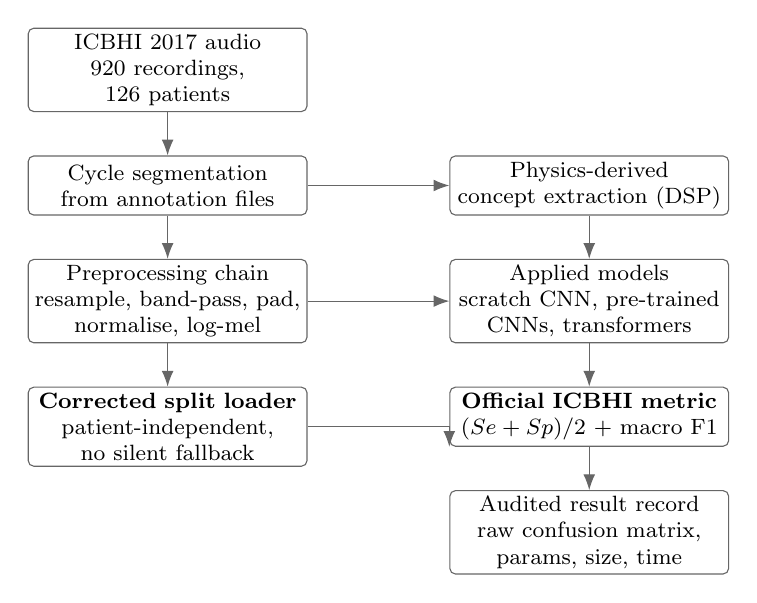
\begin{tikzpicture}[
  node distance=5.5mm and 7mm,
  every node/.style={font=\footnotesize},
  box/.style={rectangle, rounded corners=2pt, draw=black!60, align=center,
              minimum height=7.5mm, text width=34mm, inner sep=2pt},
  gate/.style={box, draw=black!80, thick},
  arr/.style={-{Latex[length=2mm]}, draw=black!60}]

\node[box] (raw) {ICBHI 2017 audio\\920 recordings, 126 patients};
\node[box, below=of raw] (seg) {Cycle segmentation\\from annotation files};
\node[box, below=of seg] (pre) {Preprocessing chain\\resample, band-pass, pad,\\normalise, log-mel};
\node[box, below=of pre] (split) {\textbf{Corrected split loader}\\patient-independent,\\no silent fallback};

\node[box, right=18mm of pre] (models) {Applied models\\scratch CNN, pre-trained\\CNNs, transformers};
\node[box, above=of models] (concept) {Physics-derived\\concept extraction (DSP)};
\node[box, below=of models] (metrics) {\textbf{Official ICBHI metric}\\$(Se+Sp)/2$ + macro F1};
\node[box, below=of metrics] (audit) {Audited result record\\raw confusion matrix,\\params, size, time};

\draw[arr] (raw) -- (seg);
\draw[arr] (seg) -- (pre);
\draw[arr] (pre) -- (split);
\draw[arr] (pre) -- (models);
\draw[arr] (seg.east) -- ++(0.5,0) |- (concept.west);
\draw[arr] (split.east) -| (metrics.south west) ;
\draw[arr] (concept) -- (models);
\draw[arr] (models) -- (metrics);
\draw[arr] (metrics) -- (audit);
\end{tikzpicture}
\caption{Flowchart of the complete proposed system. The two heavy-ruled blocks are
the corrected split loader and the official metric; every result reported in
Section~\ref{sec:results} passes through both, and the audited result record is the
only accepted output of an experiment.}
\label{fig:flowchart}
\end{figure}

\subsection{Dataset}
\label{subsec:dataset}

We use the ICBHI 2017 Respiratory Sound Database~\cite{rocha2019icbhi}, which
contains 920 annotated auscultation recordings from 126 patients, acquired with four
different stethoscope models at seven chest locations. Each recording is annotated
into respiratory cycles, and each cycle carries two binary flags---crackle present
and wheeze present---which combine into the four-class sound-event task used
throughout this paper: Normal, Crackle, Wheeze, and Both. The corpus contains 6{,}898
annotated cycles.

The database ships an official train/test list, and its provenance turns out to
matter more than its contents. Table~\ref{tab:splits} states the three partitions
that appear in this work. The published list assigns \emph{recordings}, not patients,
and two patients---156 and 218---have recordings on both sides of it, so it is not
patient independent despite being universally described as such. Our corrected
partition takes the published list and moves every recording of a leaking patient
into training, which is the conservative direction: the test set is then guaranteed
to contain no patient the model saw during training. The correction costs 12 of 381
test recordings, or 3.1\%, and moves the ratio from 58.6/41.4 to 59.9/40.1, closer to
the nominal 60/40. The third partition is not a design at all but a fault, described
in Section~\ref{subsec:split_audit}.

\begin{table}[!t]
\centering
\caption{The three train/test partitions appearing in this work. Only the second is
used for new results; the third is a fault, retained here because a large part of the
project's existing results were produced under it.}
\label{tab:splits}
\begin{tabular}{lrrrrl}
\toprule
Partition & Train & Test & Test \% & Test patients & Patient-independent? \\
\midrule
Official (published) & 539 & 381 & 41.4 & 49 & No --- 2 patients leak \\
Corrected (ours) & 551 & 369 & 40.1 & 47 & Yes \\
Identifier fallback & --- & --- & 7.1 & 11 & Yes, but not the official split \\
\bottomrule
\end{tabular}

\vspace{2pt}
\footnotesize Counts are recordings. The fallback rule assigned every patient with
identifier $\leq 111$ to test, yielding 492 of 6{,}898 cycles.
\end{table}

Table~\ref{tab:classdist} gives the class composition of the two test partitions that
carry results in this paper. The imbalance is severe and it is the reason every model
in this work trains with an inverse-frequency class-weighted loss: on the official
test partition the Both class holds 143 cycles against 1{,}579 Normal.

\begin{table}[!t]
\centering
\caption{Class distribution of the test partitions, recovered from the committed raw
confusion matrices of the corresponding runs.}
\label{tab:classdist}
\begin{tabular}{lrrrrr}
\toprule
Test partition & Normal & Crackle & Wheeze & Both & Total \\
\midrule
Official split & 1{,}579 & 649 & 385 & 143 & 2{,}756 \\
Identifier fallback & 255 & 164 & 38 & 35 & 492 \\
\bottomrule
\end{tabular}

\vspace{2pt}
\footnotesize Training partitions hold 4{,}025 and 6{,}406 cycles respectively. The
concept-extraction experiment of Section~\ref{subsec:conceptgate} runs on the
corrected partition (4{,}251 train / 2{,}636 test cycles, 79 / 47 patients) and
retains each cycle's true duration rather than padding it.
\end{table}

\subsection{Dataset Preprocessing}
\label{subsec:preprocessing}

All models consume the same log-mel representation, fixed once so that backbones
remain comparable. Audio is loaded and resampled to $f_s = 16$~kHz mono. Cycles are
cut from the annotation files' start and end times; the cycle is the unit of
classification, while the \emph{patient} is the unit of splitting. Each cycle is
standardised to $T = 8.0$~s by cyclic repetition when shorter and centre-cropping
when longer. Cyclic repetition is a deliberate choice over zero-padding, because
silence changes the temporal statistics that crackle-rate features depend on; it is
one of the rows of the preprocessing ablation in Section~\ref{subsec:ablation}.

The standardised waveform $x[n]$ is transformed to a mel spectrogram with a
1024-point FFT, a 400-sample (25~ms) Hann window, a 160-sample (10~ms) hop, and $M =
128$ mel filters spanning 50--2000~Hz, which covers the diagnostic band for crackles
and wheezes while rejecting most low-frequency handling noise. Writing $X[m,k]$ for
the short-time Fourier transform and $H_j[k]$ for the $j$-th mel filter, the log-mel
representation is

\begin{equation}
\label{eq:logmel}
S[j,m] = 10 \log_{10}\!\left( \sum_{k} H_j[k]\,\bigl| X[m,k] \bigr|^{2} + \epsilon \right),
\end{equation}

\noindent with $\epsilon$ a small constant guarding the logarithm. Each spectrogram is
then standardised to zero mean and unit variance,

\begin{equation}
\label{eq:standardize}
\tilde{S}[j,m] = \frac{S[j,m] - \mu_S}{\sigma_S + \epsilon},
\end{equation}

\noindent and, for the ImageNet-initialised backbones, replicated across three
channels and re-normalised with the ImageNet channel statistics.

Class imbalance is handled in the loss rather than by resampling, so that the
effective training distribution is identical across backbones. With $C = 4$ classes,
$N_c$ training cycles in class $c$, and $N = \sum_c N_c$, the weights and objective
are

\begin{equation}
\label{eq:weights}
w_c = \frac{N}{C \, N_c},
\qquad
\mathcal{L} = -\frac{1}{B}\sum_{i=1}^{B} w_{y_i} \log \hat{p}_{i,y_i},
\end{equation}

\noindent where $\hat{p}_{i,y_i}$ is the predicted probability of the true class of
cycle $i$ in a batch of size $B$. Every model in Table~\ref{tab:baselines} uses
(\ref{eq:weights}) unchanged, which is what makes the backbone comparison fair.

Augmentation is applied to the training partition only, never to validation or test.
The augmented runs use SpecAugment---two frequency masks of at most 24 of the 128 mel
bins and two time masks of at most 80 of the 801 frames---applied to
$\tilde{S}$ at load time, with the clean and augmented runs sharing seed 42 so that
the difference between them isolates the augmentation.

\pending{The band-pass filter, silence trimming, spectral-gating denoising and
per-cycle amplitude normalisation are specified in the project protocol but are not
yet implemented in the committed notebooks. Either implement and re-run, or delete
them from this subsection --- do not describe a stage the code does not perform.}

\subsection{Applied Models}
\label{subsec:models}

The model suite spans four families, assigned one primary model per group member.

\emph{Trained-from-scratch convolutional baselines.} A four-block 2D convolutional
network with 32 base channels and 0.3 dropout (421{,}732 parameters) establishes the
floor. It is included because a pre-trained backbone that cannot beat it is not
earning its transfer.

\emph{Pre-trained convolutional backbones.} MobileNetV2 and DenseNet121, both
ImageNet-initialised, fully fine-tuned, with the single-channel log-mel replicated to
three channels. The MobileNetV2 configuration was selected by a two-fold
patient-grouped architecture search over six candidates (MobileNetV3-Small/Large,
MobileNetV2, DenseNet121, and two further variants), scored by mean validation
performance across folds, so the backbone choice is itself a measured decision rather
than a default.

\emph{Transformer backbones.} \pending{Four pre-trained transformer backbones --- ViT-B/16
(Barshon), Swin-T (Farhana), DeiT-S or CvT-13 (Sami), and an AST re-run with a committed
result record (Asif) --- are required by the course specification and are not yet
complete. Fixed settings for comparability: 128$\times$801 log-mel resized to the model's
native resolution, three-channel replication with ImageNet normalisation, the same
class-weighted loss as (3), seed 42, AdamW at 1e-4 backbone / 1e-3 head, cosine
schedule, at most 40 epochs, early stopping on validation macro F1; clean run first,
then the SpecAugment pair.}

\emph{Physics-derived concept extractors.} Nine acoustic quantities are computed per
cycle directly from the waveform by digital signal processing, with no learned
parameters: crackle and wheeze scores, crackle fine ratio, crackle rate, wheeze
pitch, a rhonchi score, inspiratory fraction, spectral flatness, and temporal
peak-to-average power ratio. Only two of the nine---crackle presence and wheeze
presence---have a ground truth in ICBHI. Five are proxies for clinical entities the
database does not label, and two are descriptive. That 2/5/2 partition is itself a
result about what this benchmark can validate, and we name the proxies as
physics-derived quantities rather than after the clinical entities they approximate.

Alongside these, the project carries a set of extension models---dynamic multi-task
loss weighting, demographic feature fusion, temporal transformer aggregation over
cycles, curriculum pacing, a physics-informed auxiliary loss, low-rank adapter
fine-tuning, multistage distillation, and an open-set scorer suite---reported in
Section~\ref{subsec:novelty}. These were run under an earlier 70/30 partition and are
therefore reported separately and never ranked against the 60/40 results.

\subsection{Corrected Evaluation Protocol}
\label{subsec:protocol}

The ICBHI 2017 challenge score is a two-term average over \emph{pooled} abnormality.
Let the confusion matrix be $\mathbf{C}$ with rows indexed by truth, class $0$ being
Normal. Specificity is the Normal recall and sensitivity is the pooled recall over
the three abnormal classes:

\begin{equation}
\label{eq:official}
Sp = \frac{C_{00}}{\sum_{j} C_{0j}},
\quad
Se = \frac{\sum_{i=1}^{3} C_{ii}}{\sum_{i=1}^{3}\sum_{j} C_{ij}},
\quad
\mathrm{ICBHI} = \frac{Se + Sp}{2}.
\end{equation}

The quantity we had been reporting instead was the macro average of the per-class
recalls and the macro average of the per-class specificities:

\begin{equation}
\label{eq:macro}
\mathrm{ICBHI}_{\text{macro}}
= \frac{1}{2}\left( \frac{1}{C}\sum_{c} \mathrm{Rec}_c + \frac{1}{C}\sum_{c} \mathrm{Spec}_c \right).
\end{equation}

Equations (\ref{eq:official}) and (\ref{eq:macro}) differ in a way that is not a
constant offset. In (\ref{eq:macro}) each per-class specificity counts true negatives
drawn from the other three classes, so a rare class such as Wheeze or Both scores
close to 0.95 almost regardless of whether the model detects it at all. The
inflation is therefore largest exactly where the model is worst, and we quantify it
per run as

\begin{equation}
\label{eq:delta}
\Delta = \mathrm{ICBHI}_{\text{macro}} - \mathrm{ICBHI}.
\end{equation}

Three protocol rules follow from this and are enforced repository-wide. Every run
commits its raw confusion matrix, so that any reported score can be recomputed by a
reader; a score without a matrix is treated as unverifiable and is excluded from
every table in this paper. Every run records the provenance of its split by name, and
a notebook that cannot locate the official split file raises rather than falling back.
Every run records parameter count, on-disk size, and wall-clock training time, so
that accuracy claims can be read against their cost.

For the concept extractors, validity is assessed by the area under the receiver
operating characteristic curve against the binary crackle and wheeze flags, with
DeLong 95\% confidence intervals. The gate was pre-registered as

\begin{equation}
\label{eq:gate}
\text{pass} \iff \mathrm{AUROC} \geq 0.65 \;\wedge\; \mathrm{CI}_{\text{lo}} > 0.5 ,
\end{equation}

\noindent evaluated once per run on the test partition. The explicit AUROC floor in
(\ref{eq:gate}) matters: an earlier version of the rule required only that the
confidence interval exclude chance, and at $n \approx 2{,}600$ that condition is
satisfied by an AUROC of 0.52, which is statistically significant and practically
useless. A gate that cannot fail is not a gate.

%=======================================================================
\section{Results and Discussion}
\label{sec:results}

\subsection{Metric Audit}
\label{subsec:metric_audit}

Table~\ref{tab:metricaudit} recomputes the official score from the committed raw
confusion matrix of every run in the project that reports one, and
Fig.~\ref{fig:inflation} plots the same comparison. Across fifteen verifiable runs the
mean inflation is $\Delta = 0.1084$, the maximum is $0.2176$, and the minimum is
$0.0085$.

\begin{table}[!t]
\centering
\caption{Metric audit. Every row is recomputed from that run's committed raw
confusion matrix using (\ref{eq:official}). ``Reported'' is the macro variant of
(\ref{eq:macro}) that the run originally recorded.}
\label{tab:metricaudit}
\begin{tabular}{llrrrrr}
\toprule
Run & Split & Reported & \best{Official} & $\Delta$ & $Se$ & $Sp$ \\
\midrule
M35    & 70/30    & 0.7839 & \best{0.6864} & 0.0975 & 0.6980 & 0.6747 \\
M37    & 70/30    & 0.7969 & \best{0.6753} & 0.1216 & 0.7517 & 0.5989 \\
M35-v2 & 70/30    & 0.7918 & \best{0.6719} & 0.1199 & 0.7401 & 0.6036 \\
M22    & fallback & 0.7077 & \best{0.6495} & 0.0582 & 0.5696 & 0.7294 \\
M1     & fallback & 0.7181 & \best{0.6143} & 0.1038 & 0.3502 & 0.8784 \\
M12    & fallback & 0.7227 & \best{0.6138} & 0.1089 & 0.6118 & 0.6157 \\
M2     & fallback & 0.7227 & \best{0.6138} & 0.1089 & 0.6118 & 0.6157 \\
M30-v2 & fallback & 0.6777 & \best{0.5975} & 0.0802 & 0.4852 & 0.7098 \\
M3     & fallback & 0.6984 & \best{0.5895} & 0.1089 & 0.5359 & 0.6431 \\
M33-v2 & 70/30    & 0.6806 & \best{0.5832} & 0.0974 & 0.6190 & 0.5473 \\
M34    & 70/30    & 0.7046 & \best{0.5754} & 0.1292 & 0.6340 & 0.5168 \\
M31    & 70/30    & 0.6377 & \best{0.5535} & 0.0842 & 0.5456 & 0.5614 \\
M36    & 70/30    & 0.5137 & \best{0.5052} & 0.0085 & 0.0932 & 0.9171 \\
M32    & 70/30    & 0.6547 & \best{0.4733} & 0.1814 & 0.5721 & 0.3745 \\
M33    & 70/30    & 0.5506 & \best{0.3330} & 0.2176 & 0.6660 & 0.0000 \\
\midrule
\multicolumn{4}{l}{Mean inflation} & 0.1084 & & \\
\bottomrule
\end{tabular}

\vspace{2pt}
\footnotesize Two further runs report a score but commit no confusion matrix and are
therefore excluded as unverifiable. One disease-head run is excluded because the
challenge score is a sound-event metric and does not apply to it.
\end{table}

\begin{figure}[!t]
\centering
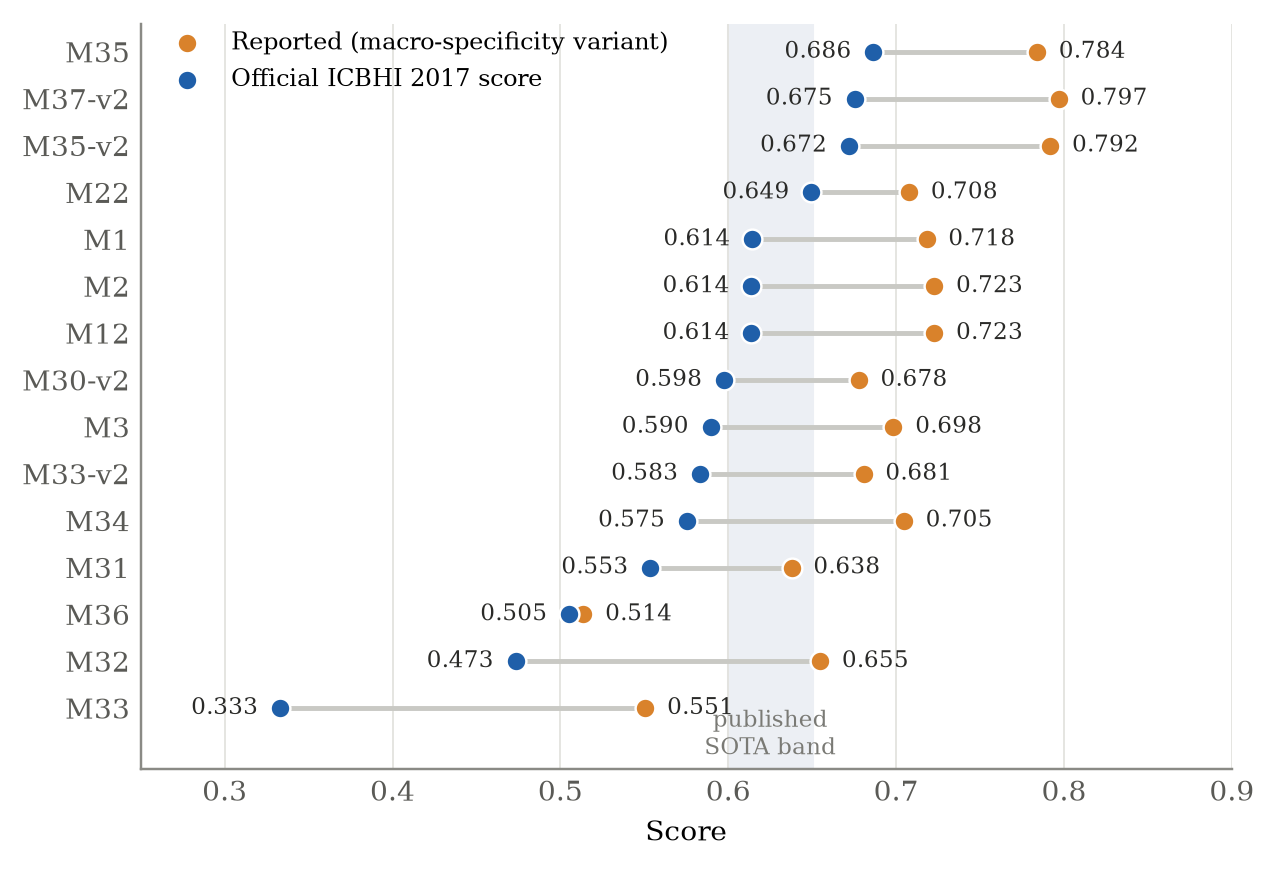
\includegraphics[width=0.92\linewidth]{fig_metric_inflation.png}
\caption{Reported versus official ICBHI score for the fifteen verifiable runs of
Table~\ref{tab:metricaudit}, sorted by the official score. The shaded band marks the
published state of the art on this benchmark. Under the macro variant, eleven of
fifteen runs appear to sit at or above the top of that band; under the official
metric, one does.}
\label{fig:inflation}
\end{figure}

Two observations matter more than the mean. The first is that the inflation is
\emph{not} a uniform rescaling, so it does not cancel in a comparison: the largest
correction (0.2176) and the smallest (0.0085) belong to two runs whose reported
scores differ by only 0.037. Ranking models by the macro variant can therefore
reorder them relative to the official metric.

The second is that the macro variant \emph{masks pathologies}. Run M33 reported
0.5506, which reads as a mediocre but working model; its official score is 0.3330
because its specificity is exactly 0.0000---the model never once predicted Normal. Run
M36 reported 0.5137 with a sensitivity of 0.0932, detecting fewer than one in ten
abnormal cycles. Both are collapses, and both are invisible in the reported column.
This is the practical argument for (\ref{eq:official}) over (\ref{eq:macro}): the
official metric is not merely the conventional one, it is the one that fails loudly.

\subsection{Split Audit}
\label{subsec:split_audit}

The second fault is more consequential than the first. Every model in one workstream
recorded its split as \texttt{patient\_independent\_official\_60\_40} while executing
a fallback rule that assigned every patient with identifier $\leq 111$ to test. The
official split file was absent from the cloud runtime and the fallback was silent.
The resulting test partition held 11 patients and 492 of 6{,}898 cycles---7.1\% of
the data, not 40\%.

Table~\ref{tab:baselines} shows what that costs. On the fallback partition the
backbone suite spans 0.5895 to 0.6495, which sits squarely inside the 0.60--0.65 band
reported by the published literature. The only two architectures we have so far
evaluated on the true official partition score 0.4139 and 0.4490---roughly twenty
points lower, and far below anything the field reports.

\begin{table}[!t]
\centering
\caption{Backbone baselines and their cost, grouped by test partition. Scores are the
official metric of (\ref{eq:official}). The two partitions must not be compared
row-for-row; see the discussion below.}
\label{tab:baselines}
\begin{tabular}{llrrrrrrr}
\toprule
Run & Backbone & ICBHI & $Se$ & $Sp$ & Acc. & F1$_{\text{macro}}$ & Params & s/epoch \\
\midrule
\multicolumn{9}{l}{\emph{Identifier-fallback partition (11 test patients, 492 cycles)}}\\
M1     & 2D CNN (scratch)        & 0.6143 & 0.3502 & 0.8784 & 0.5407 & 0.4844 & 421{,}732   & 167.4 \\
M2/M12 & 2D CNN (tuned)          & 0.6138 & 0.6118 & 0.6157 & 0.6138 & 0.5238 & 3{,}627{,}476 & 30.1 \\
M3     & MobileNetV2             & 0.5895 & 0.5359 & 0.6431 & 0.5915 & 0.4904 & 2{,}228{,}996 & 30.5 \\
M22    & MobileNetV2 + SpecAug.  & \best{0.6495} & 0.5696 & 0.7294 & 0.6524 & 0.5253 & 2{,}228{,}996 & 31.4 \\
M30-v2 & Gated M2+M3 fusion      & 0.5975 & 0.4852 & 0.7098 & 0.6016 & 0.4675 & 7{,}957{,}724 & --- \\
\midrule
\multicolumn{9}{l}{\emph{Official partition (49 test patients, 2{,}756 cycles)}}\\
M2     & 2D CNN (scratch)        & 0.4139 & 0.5030 & 0.3249 & 0.4009 & 0.3597 & 421{,}732   & 13.2 \\
M3     & DenseNet121             & \best{0.4490} & 0.4902 & 0.4079 & 0.4430 & 0.3816 & 6{,}957{,}956 & 50.1 \\
\bottomrule
\end{tabular}

\vspace{2pt}
\footnotesize All runs: Tesla T4, seed 42, class-weighted loss of (\ref{eq:weights}),
40 epochs. The two official-partition scores were recomputed by us from committed
confusion matrices; they were not present in the original records.
\end{table}

We state the limit of this comparison plainly, because it is the paper's most
attackable claim. The two partitions do not carry the same architectures: the
official-partition rows are a scratch CNN and DenseNet121, while the fallback rows
are dominated by MobileNetV2 variants. The twenty-point gap therefore conflates
partition difficulty with architecture, and cannot be attributed to the split alone
on this evidence. What can be said without qualification is narrower and still
serious: a 7.1\% test partition drawn from 11 patients was recorded, for months, as a
40\% official partition, and every score computed on it was read against a literature
that used the real thing. \pending{Re-run M2, M3 and M22 unchanged on the corrected
partition. This is the single highest-value remaining experiment in the project: it
converts the paragraph above from a caveat into a matched, one-variable measurement.}

The third fault is a property of the benchmark rather than of our code. The published
split list assigns recordings, so patient 156 contributes 9 training and 8 test
recordings and patient 218 contributes 4 and 4. Any work describing the published
ICBHI split as patient-independent is, strictly, describing something else. Our
corrected loader reports both modes, refuses to call the corrected one ``official'',
and raises rather than substituting a fallback when the split file is missing.

\subsection{Effect of Data Augmentation}
\label{subsec:augmentation}

Table~\ref{tab:augmentation} isolates SpecAugment. The clean and augmented runs share
the backbone, the parameter count, the loss, the seed and the partition, so the
difference between them is attributable to the augmentation alone.

\begin{table}[!t]
\centering
\caption{Effect of SpecAugment on the training partition only. One variable changed.}
\label{tab:augmentation}
\begin{tabular}{llrrrr}
\toprule
Run & Configuration & ICBHI & $Se$ & $Sp$ & F1$_{\text{macro}}$ \\
\midrule
M3  & MobileNetV2, clean        & 0.5895 & 0.5359 & 0.6431 & 0.4904 \\
M22 & MobileNetV2 + SpecAugment & \best{0.6495} & 0.5696 & 0.7294 & 0.5253 \\
\midrule
    & $\Delta$                  & \best{+0.0600} & +0.0337 & +0.0863 & +0.0349 \\
\bottomrule
\end{tabular}
\end{table}

SpecAugment is the project's most reliable single intervention, worth $+0.0600$
official score, and it improves specificity roughly two and a half times as much as
sensitivity. That asymmetry is worth noting rather than glossing: masking makes the
model more conservative about calling a cycle abnormal, which raises the metric on
this class distribution but is the opposite of what a screening application wants.
\pending{Repeat this clean-versus-augmented pair for each of the four transformer
backbones once they exist; the paired $\Delta$ column is what the course requirement
asks for and what makes the augmentation claim general rather than anecdotal.}

\subsection{Extension Models}
\label{subsec:novelty}

Table~\ref{tab:novelty} reports the extension suite. Every row was produced under an
earlier 70/30 patient-independent partition (38 test patients, 2{,}749 cycles) and is
therefore \emph{not} comparable to Table~\ref{tab:baselines}. We give the partition
its own column rather than dropping the rows, because silently mixing partitions in
one table is precisely the fault Section~\ref{subsec:split_audit} is about.

\begin{table}[!t]
\centering
\caption{Extension models, all on the 70/30 partition (38 test patients, 2{,}749
cycles). Not comparable to Table~\ref{tab:baselines}.}
\label{tab:novelty}
\begin{tabular}{llrrrrrr}
\toprule
Run & Mechanism & ICBHI & $Se$ & $Sp$ & F1$_{\text{macro}}$ & Params & s/epoch \\
\midrule
M35    & Physics-informed loss      & \best{0.6864} & 0.6980 & 0.6747 & 0.6420 & 3{,}627{,}476  & 144.4 \\
M37-v2 & Low-rank adapters (PEFT)   & 0.6753 & 0.7517 & 0.5989 & 0.6599 & 3{,}635{,}700  & 136.6 \\
M35-v2 & Physics-informed loss, v2  & 0.6719 & 0.7401 & 0.6036 & 0.6491 & 3{,}627{,}476  & 140.4 \\
M33-v2 & Temporal transformer       & 0.5832 & 0.6190 & 0.5473 & 0.4948 & 13{,}186{,}008 & 152.0 \\
M34    & Curriculum pacing          & 0.5754 & 0.6340 & 0.5168 & 0.5268 & 3{,}627{,}476  & 132.8 \\
M31    & GradNorm multi-task        & 0.5535 & 0.5456 & 0.5614 & 0.4351 & 3{,}726{,}297  & 191.6 \\
M36    & Multistage distillation    & 0.5052 & 0.0932 & 0.9171 & 0.2155 & 4{,}980        & 149.3 \\
M32    & Demographic fusion         & 0.4733 & 0.5721 & 0.3745 & 0.4378 & 3{,}735{,}732  & 163.8 \\
M33    & Temporal transformer, v1   & 0.3330 & 0.6660 & 0.0000 & 0.2393 & 13{,}186{,}008 & 141.8 \\
\bottomrule
\end{tabular}
\end{table}

Three results in this table are negative and are reported as such. M32's demographic
fusion falls below every convolutional baseline, indicating that patient age and sex
as encoded here carry no usable signal for cycle-level sound events. M33's first
version collapsed to a single-class predictor ($Sp = 0.0000$); its revision recovers
to 0.5832 but still does not reach the backbone baselines, at 3.6 times the
parameters. M36 compressed the model to 4{,}980 parameters---three orders of
magnitude smaller---but detects fewer than one abnormal cycle in ten, which makes its
0.5052 an artefact of a near-constant Normal prediction rather than a compression
success.

The two positive results are more interesting for what they cost than for what they
score. M37's low-rank adapters reach 0.6753 while training a small fraction of the
parameters, which is the strongest efficiency argument in the suite. M35's
physics-informed auxiliary loss is the best number the project has produced by any
metric, but its own revision regressed to 0.6719 with a best epoch of 1---a pattern
the repository audit flags automatically, and one that should be read as instability
rather than as a second confirmation. \pending{Re-run M35 on the corrected official
partition. It is the one number that would change the story if it survives the harder
split, and it is a single job.}

\subsection{Concept Validity Gate}
\label{subsec:conceptgate}

Table~\ref{tab:gate} reports the pre-registered gate of (\ref{eq:gate}) on the two
concepts ICBHI can validate. Both runs used the corrected partition; the extractors
carry no learned parameters, so there is no training and no opportunity to fit the
test set except through the experimenter.

\begin{table}[!t]
\centering
\caption{Pre-registered concept validity gate (\ref{eq:gate}). Run 2 used extractors
revised against five diagnosed failure modes from Run 1. AUROC with DeLong 95\%
confidence intervals; AUPRC against class prevalence.}
\label{tab:gate}
\begin{tabular}{llrlrrl}
\toprule
Run & Concept & AUROC & 95\% CI & AUPRC & Prevalence & Gate \\
\midrule
1 & Crackle score & 0.5506 & [0.5260, 0.5751] & --- & 0.2667 & Fail \\
1 & Wheeze score  & 0.5729 & [0.5462, 0.5996] & --- & 0.1741 & Fail \\
2 & Crackle score & 0.5580 & [0.5329, 0.5831] & 0.3079 & 0.2667 & Fail \\
2 & Wheeze score  & 0.5340 & [0.5048, 0.5631] & 0.1903 & 0.1741 & Fail \\
\bottomrule
\end{tabular}

\vspace{2pt}
\footnotesize $n = 2{,}636$ test cycles; 703 crackle-positive, 459 wheeze-positive.
Extraction costs 55.8~ms per cycle on CPU and has zero parameters. Run 1 was scored
under an earlier confidence-interval-only rule and recorded a pass; it fails the
pre-registered rule of (\ref{eq:gate}) and is reported here as a fail.
\end{table}

Both concepts fail on both runs by a wide margin, and the AUPRC lift over prevalence
is 0.0412 for crackles and 0.0162 for wheezes---barely above what a constant
predictor achieves. The diagnostics are more informative than the headline. The Run~1
extractors saturated: crackle rate averaged 10.16~Hz, which is not a plausible
physiological crackle density, and the wheeze score was exactly zero for the median
cycle, silent on roughly half the wheeze-positive cycles. The Run~2 revisions fixed
both mechanisms---crackle rate fell to 3.05~Hz and the wheeze median rose to
0.596---and each fix traded one failure mode for its opposite: the wheeze detector
went from silent on half the wheeze cycles to firing on nearly all cycles, and the
crackle AUROC moved by 0.0074 while the wheeze AUROC \emph{fell} by 0.0389. The fine
crackle ratio never functioned on real audio at all, remaining at a median of zero
across both runs.

\textbf{We stopped after two runs.} The test partition had then been read twice, and a
third revision aimed at this gate would have been fitting it; any resulting pass would
have been uninterpretable. This is the methodological spine of the result, and it is
worth more than a marginal pass would have been.

Two things must be kept separate in reading this. Our extractors are weak---that is
demonstrated, twice. Whether the 0.65 threshold is reachable on this reference
standard by \emph{any} method is a different question, and this experiment cannot
decide it. Section~\ref{subsec:ceiling} is why that distinction matters.

\subsection{The Label-Reliability Ceiling}
\label{subsec:ceiling}

Table~\ref{tab:human} collects the published human reference points for this exact
task. They reframe the previous subsection.

\begin{table}[!t]
\centering
\caption{Human performance and agreement on respiratory sound labelling.}
\label{tab:human}
\begin{tabular}{llr}
\toprule
Source & Measurement & Value \\
\midrule
Tzeng \emph{et al.}~\cite{tzeng2025jmir} & 7 physicians, ICBHI score, clean audio & 47.77\% \\
                                          & \quad sensitivity & 23.23\% \\
                                          & \quad specificity & 72.32\% \\
                                          & \quad self-rated confidence (of 5) & 2.88 \\
\midrule
Aviles-Solis \emph{et al.}~\cite{aviles2016kappa} & 12 physicians, detailed descriptions & $\kappa < 0.40$ \\
                                          & \quad collapsed to ``crackles'' & $\kappa = 0.62$ \\
                                          & \quad collapsed to ``wheezes'' & $\kappa = 0.59$ \\
\bottomrule
\end{tabular}
\end{table}

Seven senior physicians, blind, on clean ICBHI audio, reach an ICBHI score of 47.77\%
and miss roughly 77\% of the cycles the database marks abnormal. Our best backbone on
the fallback partition scores 0.6495 and our best on the true partition 0.4490; the
latter is close to the physician figure. Read alone, a 0.5580 concept AUROC looks like
failure. Read against a reference standard that experts reproduce this poorly, it
looks like a measurement of the reference standard.

The agreement data sharpens the point. Our fine crackle ratio was targeting the
fine-versus-coarse distinction, on which twelve physicians agree at $\kappa < 0.40$.
Its ceiling was set before a line of signal processing was written. Collapsing to
presence-only categories raises agreement to $\kappa \approx 0.6$, which is exactly
the boundary between the two of our nine concepts that ICBHI can validate and the
five that it cannot.

We scope the claim deliberately. We are not claiming that ICBHI's labels are wrong,
that the benchmark should be abandoned, or that concept-based methods cannot work for
auscultation. We claim that concept-level validation \emph{against these cycle
labels} is bounded in a way the literature does not currently report, and we supply
the protocol and tooling to measure that bound.

\pending{Our own clinician listening study --- one physician, 120 blind clips plus 12
hidden duplicates, shipped with six calibration exemplars that the published
seven-physician study did not report providing --- is in flight. When the labels
return, add: intra-rater agreement from the hidden duplicates, clinician-versus-ICBHI
agreement, and the first fine/coarse crackle reference on this corpus. State the
$n=1$ limitation explicitly; the published $n=7$ and $n=12$ studies carry the
reliability argument, and ours adds the fine-grained reference neither has.}

\subsection{Open-Set Behaviour}
\label{subsec:openset}

Table~\ref{tab:openset} reports patient-level unknown-detection scores with bootstrap
confidence intervals.

\begin{table}[!t]
\centering
\caption{Patient-level unknown-disease detection. 19 unknown and 42 known patients.}
\label{tab:openset}
\begin{tabular}{llrl}
\toprule
Run & Scorer & AUROC & 95\% CI \\
\midrule
M29    & Energy                 & 0.6466 & [0.4917, 0.8015] \\
M29    & Entropy                & 0.5789 & [0.4206, 0.7372] \\
M29    & Mahalanobis            & 0.5689 & --- \\
M15-v6 & Cross-task disagreement& 0.5747 & [0.4163, 0.7331] \\
M14-v2 & Conformal wrapper      & 0.4809 & [0.3019, 0.6599] \\
\bottomrule
\end{tabular}
\end{table}

Every interval in Table~\ref{tab:openset} spans 0.5. With 19 unknown patients the
study is underpowered, and the correct statement is that \emph{no scorer here has
been shown to beat chance}---not that the energy score is best. We report it this way
because the alternative phrasing, which the ranking invites, would be the same class
of error as Section~\ref{subsec:metric_audit}: a number presented at a precision the
evidence does not support. The cross-task disagreement scorer, which was the
project's original headline mechanism, does not outperform the energy baseline.

\subsection{Interpretability Analysis}
\label{subsec:xai}

\pending{No interpretability analysis exists yet. Build one notebook producing, for
the best model under the corrected partition: (i) Grad-CAM over the final
convolutional block, overlaid on the log-mel spectrogram; (ii) occlusion sensitivity
as a model-agnostic cross-check; (iii) a four-panel figure with one correctly
classified example of each class plus at least one misclassification. The analysis
that lifts this above decoration: ICBHI annotates crackle and wheeze event
\emph{times}, so measure whether the Grad-CAM mass falls inside the annotated event
window and report that pointing-game hit rate as a number. Given this paper's own
finding, phrase the result as evidence about where the model looks, never as clinical
validation.}

\begin{figure}[!t]
\centering
\fbox{\begin{minipage}[c][4cm][c]{0.9\linewidth}\centering
\textit{Fig.~5 --- interpretability panel, pending}\end{minipage}}
\caption{Grad-CAM and occlusion-sensitivity maps for the best model, with the
pointing-game hit rate against annotated event windows. \pending{figure}}
\label{fig:xai}
\end{figure}

\subsection{Best Model and Ablation Study}
\label{subsec:ablation}

We define the best model once, in advance, to avoid selecting it after the fact:
\emph{the highest official ICBHI score on the corrected 60/40 partition, among runs
that commit a raw confusion matrix}. Under that rule the current best is M22,
MobileNetV2 with SpecAugment, at 0.6495---with the caveat, carried explicitly from
Section~\ref{subsec:split_audit}, that this score is on the fallback partition and
must be re-established once the corrected re-runs land. M35's 0.6864 is on the 70/30
partition and cannot be ranked against it; we say so rather than quietly promoting it.

Fig.~\ref{fig:cm} and Fig.~\ref{fig:curves} give the required diagnostics for that
model. The confusion matrix shows where the imbalance bites: Normal and Crackle are
recovered at 0.729 and 0.640, while Both---35 test cycles---reaches 0.286, with most
of its mass falling into Wheeze and Crackle. The training curves show a clean
overfitting signature, with validation loss reaching its minimum at epoch 9 and
rising monotonically thereafter while training loss continues to fall; early stopping
on the validation metric is doing real work here, and a report of the final-epoch
model would have been substantially worse.

\begin{figure}[!t]
\centering
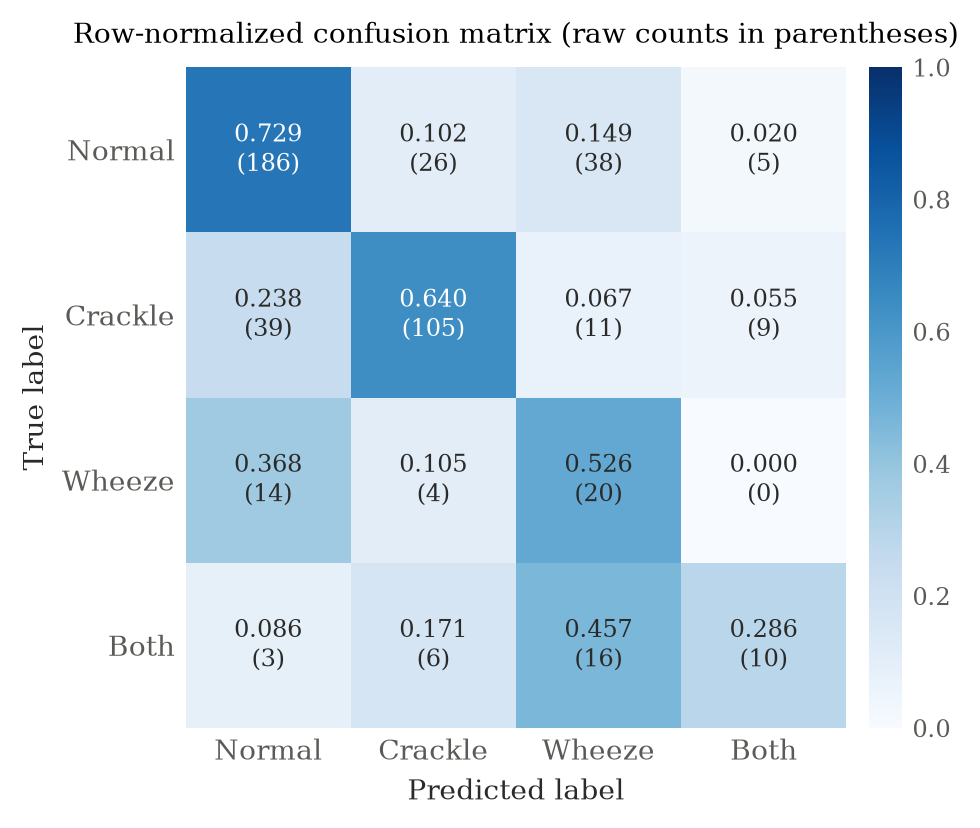
\includegraphics[width=0.66\linewidth]{fig_confusion_best.png}
\caption{Row-normalized confusion matrix of the best model (M22, MobileNetV2 +
SpecAugment), with raw counts in parentheses. Test partition: 492 cycles.}
\label{fig:cm}
\end{figure}

\begin{figure}[!t]
\centering
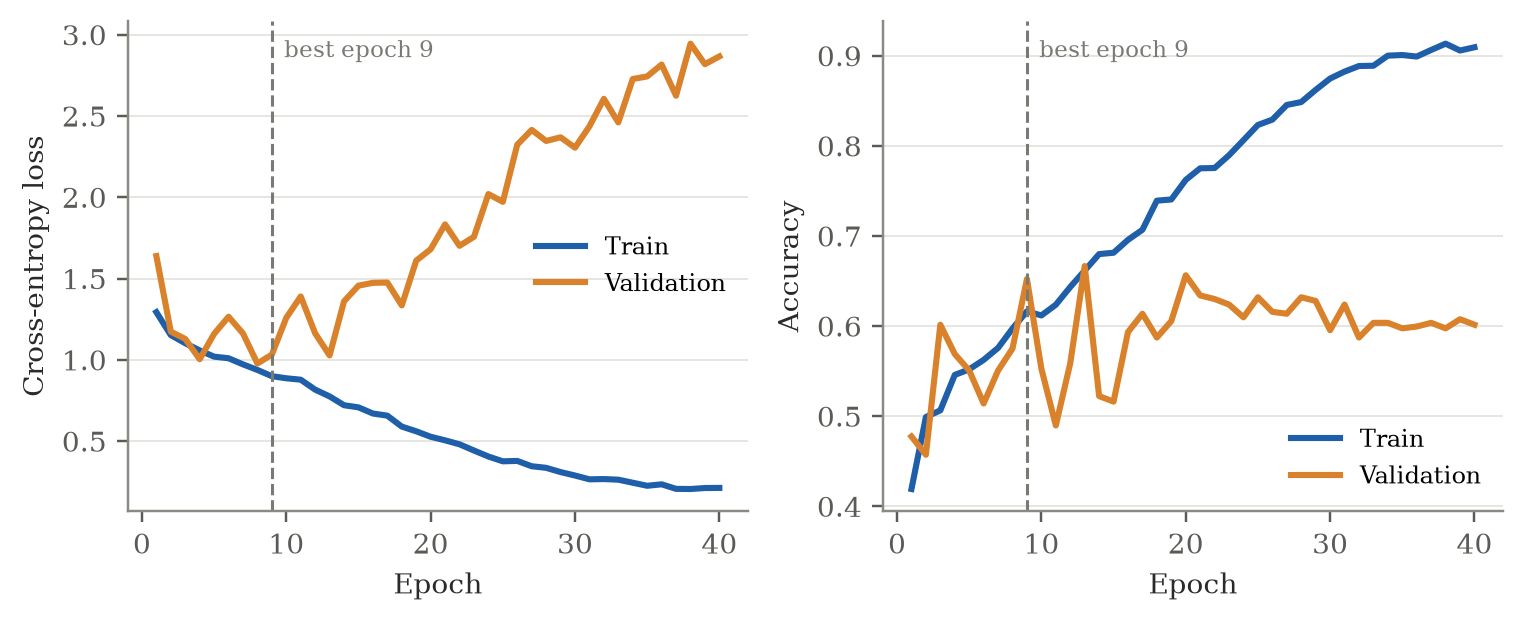
\includegraphics[width=\linewidth]{fig_curves_best.png}
\caption{Training and validation loss (left) and accuracy (right) versus epoch for the
best model. The dashed line marks the selected epoch. Validation loss diverges from
epoch 9 onward while training loss continues to fall.}
\label{fig:curves}
\end{figure}

Table~\ref{tab:ablation} is the ablation study. One row exists as a completed
one-variable experiment; the remainder are specified and pending. We list them
in the table rather than omitting them so that the design is auditable and the
missing evidence is visible.

\begin{table}[!t]
\centering
\caption{Component-wise and preprocessing ablation on the best model. One variable
changed per row, all on the corrected partition.}
\label{tab:ablation}
\begin{tabular}{llrrl}
\toprule
Row & Change from full model & ICBHI & $\Delta$ & Isolates \\
\midrule
A0 & Full model (reference)          & 0.6495 & ---      & --- \\
A1 & $-$ SpecAugment                 & 0.5895 & $-0.0600$ & Augmentation \\
A2 & $-$ ImageNet initialisation     & \pending{run} & & Transfer learning \\
A3 & $-$ class-weighted loss         & \pending{run} & & Imbalance handling \\
A4 & Frozen backbone, head only      & \pending{run} & & Value of fine-tuning \\
A5 & 64 mel bins instead of 128      & \pending{run} & & Input resolution \\
A6 & 4~s cycles instead of 8~s       & \pending{run} & & Temporal context \\
\midrule
P1 & $-$ band-pass filter            & \pending{run} & & Filtering \\
P2 & $-$ denoising                   & \pending{run} & & Noise suppression \\
P3 & $-$ amplitude normalisation     & \pending{run} & & Device gain \\
P4 & Zero-padding instead of cyclic  & \pending{run} & & Padding policy \\
P5 & $-$ spectrogram standardisation & \pending{run} & & Input scaling \\
\bottomrule
\end{tabular}

\vspace{2pt}
\footnotesize Row A1 is the completed comparison of Table~\ref{tab:augmentation}.
Report every filled row with $Se$, $Sp$, macro F1, parameters and seconds per epoch.
If a removal \emph{improves} the score, report it --- the project already carries two
regressions in its record, and that consistency is what makes the rest credible.
\end{table}

\subsection{Comparison with Existing Works}
\label{subsec:comparison}

Table~\ref{tab:comparison} places this work against the literature. We report our
official-metric scores only, and we report the partition for every row, because the
argument of this paper is that a comparison without those two columns is not a
comparison.

\begin{table}[!t]
\centering
\caption{Comparison of the proposed system with existing work on ICBHI 2017. All
scores are the official challenge metric of (\ref{eq:official}).}
\label{tab:comparison}
\begin{tabular}{lllrl}
\toprule
Source & Method & Partition & ICBHI & Notes \\
\midrule
Suma \emph{et al.}~\cite{suma2025mtl}        & MTL MobileNet          & \pending{verify} & \pending{verify} & Closed-set MTL \\
ADFF-Net~\cite{adffnet2025}                  & AST dual-stream fusion & \pending{verify} & \pending{verify} & Attention fusion \\
Fusion~\cite{bspc2025fusion}                 & Time + 2D co-attention & \pending{verify} & \pending{verify} & Reports $+1.00\%$ \\
Cho and Lee~\cite{cho2025openset}            & Open-set prototypes    & \pending{verify} & \pending{verify} & Only open-set work \\
Tzeng \emph{et al.}~\cite{tzeng2025jmir}     & 7 senior physicians    & 25\% of test     & 0.4777 & Human reference \\
\midrule
\multirow{2}{*}{This work} & MobileNetV2 + SpecAugment & fallback  & 0.6495 & Not the official split \\
                           & DenseNet121               & official  & 0.4490 & Recomputed by us \\
\bottomrule
\end{tabular}

\vspace{2pt}
\footnotesize \pending{Fill the four verify cells from the publisher record, not from
a search result, and confirm each reported score is the official metric on a stated
partition. If a paper does not state its partition precisely, say so in the Notes
column --- that absence is itself evidence for this paper's argument.}
\end{table}

The honest reading of this table is that our corrected numbers do not lead it. That
is the point. Our uncorrected numbers would have led it, and they were wrong twice
over. A system reporting 0.7227 on a 7.1\% test partition under a non-standard metric
is not state of the art; it is an unaudited measurement, and the literature it would
have been compared against may contain the same class of error.

\subsection{Limitations}
\label{subsec:limitations}

Four limitations bound the claims above. The corrected-partition evidence currently
rests on two architectures, not a matched re-run of the full suite, so the size of the
split effect is estimated rather than measured. The concept extractors are one
implementation, and a better one may exist; we cannot separate ``our detector is
weak'' from ``0.65 is unreachable here'' from this experiment alone, and we do not try
to. The reliability argument leans on two published studies plus a single-clinician
study still in flight, against the $n=7$ and $n=12$ of the literature. And all of it
concerns one corpus: ICBHI is the field's default benchmark and the faults we describe
are ICBHI-specific, so the scope of the claim is that benchmark and no further.

%=======================================================================
\section{Conclusions}
\label{sec:conclusion}

We audited our own respiratory sound pipeline on ICBHI 2017 and found three
measurement faults, each of which independently changes what our results appear to
say. A macro-averaged variant of the challenge score inflated fifteen committed runs
by 0.1084 on average and 0.2176 at worst, and masked two outright model collapses
that the official metric exposes immediately. A silent split fallback substituted an
11-patient, 7.1\% test partition for the official 40\% one. The published official
split assigns recordings rather than patients and is not patient-independent. We
supplied corrected baselines under the official metric, a pre-registered
concept-validity gate that was run twice and failed twice under a threshold chosen so
that it \emph{could} fail, and a reading of that failure against a reference standard
that seven senior physicians reproduce at a 47.77\% ICBHI score. The contribution is a
measurement rather than a mechanism: concept-level validation against ICBHI cycle
labels is bounded by the reliability of those labels, and we release the corrected
split loader, the canonical score format with paired significance tests, and the audit
tool that detects all three faults.

Three directions follow. The first is the matched re-run: evaluating the full backbone
suite unchanged on the corrected partition converts this paper's largest caveat into a
one-variable measurement of what split provenance is actually worth, and is a
prerequisite for any ranking claim. The second is extending the reliability
measurement beyond a single clinician---a multi-rater study with published calibration
exemplars would establish whether the fine-versus-coarse crackle distinction is
learnable on this corpus at all, or whether it should be retired from concept-based
work on it. The third is applying the audit to the wider literature: the three fault
classes described here are detectable from a committed confusion matrix and a stated
partition, and a survey of how many published ICBHI systems supply either would
establish whether these are our errors or the field's.

%=======================================================================
\bibliographystyle{IEEEtran}
\bibliography{references}

\end{document}
